% Options for packages loaded elsewhere
\PassOptionsToPackage{unicode}{hyperref}
\PassOptionsToPackage{hyphens}{url}
\PassOptionsToPackage{dvipsnames,svgnames,x11names}{xcolor}
%
\documentclass[
  letterpaper,
  DIV=11,
  numbers=noendperiod]{scrartcl}

\usepackage{amsmath,amssymb}
\usepackage{iftex}
\ifPDFTeX
  \usepackage[T1]{fontenc}
  \usepackage[utf8]{inputenc}
  \usepackage{textcomp} % provide euro and other symbols
\else % if luatex or xetex
  \usepackage{unicode-math}
  \defaultfontfeatures{Scale=MatchLowercase}
  \defaultfontfeatures[\rmfamily]{Ligatures=TeX,Scale=1}
\fi
\usepackage{lmodern}
\ifPDFTeX\else  
    % xetex/luatex font selection
\fi
% Use upquote if available, for straight quotes in verbatim environments
\IfFileExists{upquote.sty}{\usepackage{upquote}}{}
\IfFileExists{microtype.sty}{% use microtype if available
  \usepackage[]{microtype}
  \UseMicrotypeSet[protrusion]{basicmath} % disable protrusion for tt fonts
}{}
\makeatletter
\@ifundefined{KOMAClassName}{% if non-KOMA class
  \IfFileExists{parskip.sty}{%
    \usepackage{parskip}
  }{% else
    \setlength{\parindent}{0pt}
    \setlength{\parskip}{6pt plus 2pt minus 1pt}}
}{% if KOMA class
  \KOMAoptions{parskip=half}}
\makeatother
\usepackage{xcolor}
\setlength{\emergencystretch}{3em} % prevent overfull lines
\setcounter{secnumdepth}{-\maxdimen} % remove section numbering
% Make \paragraph and \subparagraph free-standing
\ifx\paragraph\undefined\else
  \let\oldparagraph\paragraph
  \renewcommand{\paragraph}[1]{\oldparagraph{#1}\mbox{}}
\fi
\ifx\subparagraph\undefined\else
  \let\oldsubparagraph\subparagraph
  \renewcommand{\subparagraph}[1]{\oldsubparagraph{#1}\mbox{}}
\fi

\usepackage{color}
\usepackage{fancyvrb}
\newcommand{\VerbBar}{|}
\newcommand{\VERB}{\Verb[commandchars=\\\{\}]}
\DefineVerbatimEnvironment{Highlighting}{Verbatim}{commandchars=\\\{\}}
% Add ',fontsize=\small' for more characters per line
\usepackage{framed}
\definecolor{shadecolor}{RGB}{241,243,245}
\newenvironment{Shaded}{\begin{snugshade}}{\end{snugshade}}
\newcommand{\AlertTok}[1]{\textcolor[rgb]{0.68,0.00,0.00}{#1}}
\newcommand{\AnnotationTok}[1]{\textcolor[rgb]{0.37,0.37,0.37}{#1}}
\newcommand{\AttributeTok}[1]{\textcolor[rgb]{0.40,0.45,0.13}{#1}}
\newcommand{\BaseNTok}[1]{\textcolor[rgb]{0.68,0.00,0.00}{#1}}
\newcommand{\BuiltInTok}[1]{\textcolor[rgb]{0.00,0.23,0.31}{#1}}
\newcommand{\CharTok}[1]{\textcolor[rgb]{0.13,0.47,0.30}{#1}}
\newcommand{\CommentTok}[1]{\textcolor[rgb]{0.37,0.37,0.37}{#1}}
\newcommand{\CommentVarTok}[1]{\textcolor[rgb]{0.37,0.37,0.37}{\textit{#1}}}
\newcommand{\ConstantTok}[1]{\textcolor[rgb]{0.56,0.35,0.01}{#1}}
\newcommand{\ControlFlowTok}[1]{\textcolor[rgb]{0.00,0.23,0.31}{#1}}
\newcommand{\DataTypeTok}[1]{\textcolor[rgb]{0.68,0.00,0.00}{#1}}
\newcommand{\DecValTok}[1]{\textcolor[rgb]{0.68,0.00,0.00}{#1}}
\newcommand{\DocumentationTok}[1]{\textcolor[rgb]{0.37,0.37,0.37}{\textit{#1}}}
\newcommand{\ErrorTok}[1]{\textcolor[rgb]{0.68,0.00,0.00}{#1}}
\newcommand{\ExtensionTok}[1]{\textcolor[rgb]{0.00,0.23,0.31}{#1}}
\newcommand{\FloatTok}[1]{\textcolor[rgb]{0.68,0.00,0.00}{#1}}
\newcommand{\FunctionTok}[1]{\textcolor[rgb]{0.28,0.35,0.67}{#1}}
\newcommand{\ImportTok}[1]{\textcolor[rgb]{0.00,0.46,0.62}{#1}}
\newcommand{\InformationTok}[1]{\textcolor[rgb]{0.37,0.37,0.37}{#1}}
\newcommand{\KeywordTok}[1]{\textcolor[rgb]{0.00,0.23,0.31}{#1}}
\newcommand{\NormalTok}[1]{\textcolor[rgb]{0.00,0.23,0.31}{#1}}
\newcommand{\OperatorTok}[1]{\textcolor[rgb]{0.37,0.37,0.37}{#1}}
\newcommand{\OtherTok}[1]{\textcolor[rgb]{0.00,0.23,0.31}{#1}}
\newcommand{\PreprocessorTok}[1]{\textcolor[rgb]{0.68,0.00,0.00}{#1}}
\newcommand{\RegionMarkerTok}[1]{\textcolor[rgb]{0.00,0.23,0.31}{#1}}
\newcommand{\SpecialCharTok}[1]{\textcolor[rgb]{0.37,0.37,0.37}{#1}}
\newcommand{\SpecialStringTok}[1]{\textcolor[rgb]{0.13,0.47,0.30}{#1}}
\newcommand{\StringTok}[1]{\textcolor[rgb]{0.13,0.47,0.30}{#1}}
\newcommand{\VariableTok}[1]{\textcolor[rgb]{0.07,0.07,0.07}{#1}}
\newcommand{\VerbatimStringTok}[1]{\textcolor[rgb]{0.13,0.47,0.30}{#1}}
\newcommand{\WarningTok}[1]{\textcolor[rgb]{0.37,0.37,0.37}{\textit{#1}}}

\providecommand{\tightlist}{%
  \setlength{\itemsep}{0pt}\setlength{\parskip}{0pt}}\usepackage{longtable,booktabs,array}
\usepackage{calc} % for calculating minipage widths
% Correct order of tables after \paragraph or \subparagraph
\usepackage{etoolbox}
\makeatletter
\patchcmd\longtable{\par}{\if@noskipsec\mbox{}\fi\par}{}{}
\makeatother
% Allow footnotes in longtable head/foot
\IfFileExists{footnotehyper.sty}{\usepackage{footnotehyper}}{\usepackage{footnote}}
\makesavenoteenv{longtable}
\usepackage{graphicx}
\makeatletter
\def\maxwidth{\ifdim\Gin@nat@width>\linewidth\linewidth\else\Gin@nat@width\fi}
\def\maxheight{\ifdim\Gin@nat@height>\textheight\textheight\else\Gin@nat@height\fi}
\makeatother
% Scale images if necessary, so that they will not overflow the page
% margins by default, and it is still possible to overwrite the defaults
% using explicit options in \includegraphics[width, height, ...]{}
\setkeys{Gin}{width=\maxwidth,height=\maxheight,keepaspectratio}
% Set default figure placement to htbp
\makeatletter
\def\fps@figure{htbp}
\makeatother

\usepackage{booktabs}
\usepackage{longtable}
\usepackage{array}
\usepackage{multirow}
\usepackage{wrapfig}
\usepackage{float}
\usepackage{colortbl}
\usepackage{pdflscape}
\usepackage{tabu}
\usepackage{threeparttable}
\usepackage{threeparttablex}
\usepackage[normalem]{ulem}
\usepackage{makecell}
\usepackage{xcolor}
\usepackage{caption}
\usepackage{anyfontsize}
\KOMAoption{captions}{tableheading}
\makeatletter
\@ifpackageloaded{caption}{}{\usepackage{caption}}
\AtBeginDocument{%
\ifdefined\contentsname
  \renewcommand*\contentsname{Table of contents}
\else
  \newcommand\contentsname{Table of contents}
\fi
\ifdefined\listfigurename
  \renewcommand*\listfigurename{List of Figures}
\else
  \newcommand\listfigurename{List of Figures}
\fi
\ifdefined\listtablename
  \renewcommand*\listtablename{List of Tables}
\else
  \newcommand\listtablename{List of Tables}
\fi
\ifdefined\figurename
  \renewcommand*\figurename{Figure}
\else
  \newcommand\figurename{Figure}
\fi
\ifdefined\tablename
  \renewcommand*\tablename{Table}
\else
  \newcommand\tablename{Table}
\fi
}
\@ifpackageloaded{float}{}{\usepackage{float}}
\floatstyle{ruled}
\@ifundefined{c@chapter}{\newfloat{codelisting}{h}{lop}}{\newfloat{codelisting}{h}{lop}[chapter]}
\floatname{codelisting}{Listing}
\newcommand*\listoflistings{\listof{codelisting}{List of Listings}}
\makeatother
\makeatletter
\makeatother
\makeatletter
\@ifpackageloaded{caption}{}{\usepackage{caption}}
\@ifpackageloaded{subcaption}{}{\usepackage{subcaption}}
\makeatother
\ifLuaTeX
  \usepackage{selnolig}  % disable illegal ligatures
\fi
\usepackage{bookmark}

\IfFileExists{xurl.sty}{\usepackage{xurl}}{} % add URL line breaks if available
\urlstyle{same} % disable monospaced font for URLs
\hypersetup{
  pdftitle={Project 2},
  pdfauthor={Zhaoxiang Ding},
  colorlinks=true,
  linkcolor={blue},
  filecolor={Maroon},
  citecolor={Blue},
  urlcolor={Blue},
  pdfcreator={LaTeX via pandoc}}

\title{Project 2}
\author{Zhaoxiang Ding}
\date{}

\begin{document}
\maketitle

\subsection{Abstract}\label{abstract}

\subsection{Introduction}\label{introduction}

Behavioral activation (BA) has been viewed as a promising treatment to
address smoking cessation for individuals with major depressive disorder
(MDD),{[}@{]}. However, there are only limited study that examine the
effect of BA on smoking cessation. @ used a 2 by 2 randomized factorial
design to examine the effect of BA on smoking cessation. The study found
that BA does not have a significant effect on smoking cessation. In this
project, we will re-examine the effect of BA on smoking cessation using
the same data from @ with a different approach.

The goal of this project is to examine the potiential moderators of the
effect of behavioral treatment on end-of-treatment (EOT) abstinence and
evaluate baseline variables as predictors of abstinence, controlling for
behavioral treatment and pharmacotherapy.

\subsection{Identifing the causal
effect}\label{identifing-the-causal-effect}

In @ , work, the casual effect is identified by the difference in the
abstinence rate between the treatment group and the control group using
intent-to-treat (ITT) principles. Rather than examining the abstinence
rate, this project will examine the odds of abstinence, and the causal
effect can be identifiled by the odds ratio of abstinence between the
treatment group and the control group, using the same ITT principles.
The causal effect can be written as:

\[
\hat{\tau} &= \frac{odds(E[Y^1])}{odds(E[Y^0])}
\] The data was collected from a 2 by 2 randomized factorial design,
thus all the covariates are balanced between the treatment group and the
control group(shown in ). All the assumption of the causal effect is
satisfied. The causal effect can be written as:

\[
\begin{aligned}
\hat{\tau} &= \frac{odds(E[Y^1])}{odds(E[Y^0])} \\
&= \frac{odds(E[Y|A = 1])}{odds(E[Y|A = 0])}
\end{aligned}
\]

Rather than examining the abstinence rate, we will examine the odds of
abstinence. The odds of abstinence can be written as: We will fit the
following model to examine the effect of behaviour treatment

\[
logit(E[Y_i]) = \beta_0  + \beta_1A_i + \beta_2Z_i + \beta_3X_i^T  + \beta_4X_i^TA_i + \beta_5X_i^TZ_i +\beta_6Z_iA_i
\] Where \(A\) is the treatment group, \(X^T\) is the covariates, and
\(Y\) is the outcome. and the causal effect can be identifiled by the
following formula \[
\begin{aligned}
\tau &= \frac{odds(E[Y^1])}{odds(E[Y^0])} \\
&= \frac{odds(E[Y|A = 1])}{odds(E[Y|A = 0])} \\
&= \beta_1
\end{aligned}
\]

\subsection{Exploriatary data
analysis}\label{exploriatary-data-analysis}

\begin{Shaded}
\begin{Highlighting}[]
\FunctionTok{library}\NormalTok{(gtsummary)}
\end{Highlighting}
\end{Shaded}

\begin{verbatim}
Warning: package 'gtsummary' was built under R version 4.4.1
\end{verbatim}

\begin{Shaded}
\begin{Highlighting}[]
\FunctionTok{library}\NormalTok{(mice)}
\end{Highlighting}
\end{Shaded}

\begin{verbatim}

Attaching package: 'mice'
\end{verbatim}

\begin{verbatim}
The following object is masked from 'package:stats':

    filter
\end{verbatim}

\begin{verbatim}
The following objects are masked from 'package:base':

    cbind, rbind
\end{verbatim}

\begin{Shaded}
\begin{Highlighting}[]
\FunctionTok{library}\NormalTok{(glmnet)}
\end{Highlighting}
\end{Shaded}

\begin{verbatim}
Loading required package: Matrix
\end{verbatim}

\begin{verbatim}
Loaded glmnet 4.1-8
\end{verbatim}

\begin{Shaded}
\begin{Highlighting}[]
\FunctionTok{library}\NormalTok{(pROC)}
\end{Highlighting}
\end{Shaded}

\begin{verbatim}
Type 'citation("pROC")' for a citation.
\end{verbatim}

\begin{verbatim}

Attaching package: 'pROC'
\end{verbatim}

\begin{verbatim}
The following objects are masked from 'package:stats':

    cov, smooth, var
\end{verbatim}

\begin{Shaded}
\begin{Highlighting}[]
\FunctionTok{library}\NormalTok{(kableExtra)}
\FunctionTok{library}\NormalTok{(dplyr)}
\end{Highlighting}
\end{Shaded}

\begin{verbatim}

Attaching package: 'dplyr'
\end{verbatim}

\begin{verbatim}
The following object is masked from 'package:kableExtra':

    group_rows
\end{verbatim}

\begin{verbatim}
The following objects are masked from 'package:stats':

    filter, lag
\end{verbatim}

\begin{verbatim}
The following objects are masked from 'package:base':

    intersect, setdiff, setequal, union
\end{verbatim}

\begin{Shaded}
\begin{Highlighting}[]
\FunctionTok{library}\NormalTok{(L0Learn)}
\end{Highlighting}
\end{Shaded}

\begin{Shaded}
\begin{Highlighting}[]
\NormalTok{data }\OtherTok{\textless{}{-}} \FunctionTok{read.csv}\NormalTok{(}\StringTok{"../Data/project2.csv"}\NormalTok{)}
\NormalTok{num\_col }\OtherTok{\textless{}{-}} \FunctionTok{c}\NormalTok{(}\DecValTok{5}\NormalTok{,}\DecValTok{12}\NormalTok{,}\DecValTok{14}\SpecialCharTok{:}\DecValTok{19}\NormalTok{,}\DecValTok{23}\NormalTok{,}\DecValTok{25}\NormalTok{)}
\NormalTok{ordinal\_col }\OtherTok{\textless{}{-}} \FunctionTok{c}\NormalTok{(}\DecValTok{10}\NormalTok{,}\DecValTok{11}\NormalTok{)}
\NormalTok{data[,num\_col] }\OtherTok{\textless{}{-}} \FunctionTok{lapply}\NormalTok{(data[,num\_col], as.numeric)}
\NormalTok{data[,ordinal\_col] }\OtherTok{\textless{}{-}} \FunctionTok{lapply}\NormalTok{(data[,ordinal\_col], factor, }\AttributeTok{order =}\NormalTok{ T)}

\NormalTok{data[,}\SpecialCharTok{{-}}\FunctionTok{c}\NormalTok{(num\_col, ordinal\_col)] }\OtherTok{\textless{}{-}} \FunctionTok{lapply}\NormalTok{(data[,}\SpecialCharTok{{-}}\FunctionTok{c}\NormalTok{(num\_col, ordinal\_col)], factor)}
\end{Highlighting}
\end{Shaded}

\begin{Shaded}
\begin{Highlighting}[]
\NormalTok{data\_tbl }\OtherTok{\textless{}{-}}\NormalTok{ data[, }\SpecialCharTok{{-}}\DecValTok{1}\NormalTok{]}
\NormalTok{data\_tbl}\SpecialCharTok{$}\NormalTok{group }\OtherTok{\textless{}{-}} \FunctionTok{paste}\NormalTok{(data\_tbl}\SpecialCharTok{$}\NormalTok{Var, data\_tbl}\SpecialCharTok{$}\NormalTok{BA, }\AttributeTok{sep =} \StringTok{"\_"}\NormalTok{)}
\NormalTok{data\_tbl }\OtherTok{\textless{}{-}}\NormalTok{ data\_tbl[, }\SpecialCharTok{{-}}\FunctionTok{c}\NormalTok{(}\DecValTok{2}\NormalTok{,}\DecValTok{3}\NormalTok{)]}
\FunctionTok{tbl\_summary}\NormalTok{(data\_tbl, }\AttributeTok{by =}\NormalTok{ group)}
\end{Highlighting}
\end{Shaded}

\begingroup
\fontsize{12.0pt}{14.4pt}\selectfont
\setlength{\LTpost}{0mm}
\begin{longtable*}{lcccc}
\toprule
\textbf{Characteristic} & \textbf{0\_0}  N = 68\textsuperscript{\textit{1}} & \textbf{0\_1}  N = 68\textsuperscript{\textit{1}} & \textbf{1\_0}  N = 81\textsuperscript{\textit{1}} & \textbf{1\_1}  N = 83\textsuperscript{\textit{1}} \\ 
\midrule\addlinespace[2.5pt]
abst &  &  &  &  \\ 
    0 & 60 (88\%) & 64 (94\%) & 55 (68\%) & 57 (69\%) \\ 
    1 & 8 (12\%) & 4 (5.9\%) & 26 (32\%) & 26 (31\%) \\ 
age\_ps & 51 (45, 58) & 54 (42, 61) & 52 (41, 59) & 53 (40, 60) \\ 
sex\_ps &  &  &  &  \\ 
    1 & 29 (43\%) & 30 (44\%) & 37 (46\%) & 39 (47\%) \\ 
    2 & 39 (57\%) & 38 (56\%) & 44 (54\%) & 44 (53\%) \\ 
NHW &  &  &  &  \\ 
    0 & 46 (68\%) & 44 (65\%) & 56 (69\%) & 49 (59\%) \\ 
    1 & 22 (32\%) & 24 (35\%) & 25 (31\%) & 34 (41\%) \\ 
Black &  &  &  &  \\ 
    0 & 28 (41\%) & 31 (46\%) & 38 (47\%) & 46 (55\%) \\ 
    1 & 40 (59\%) & 37 (54\%) & 43 (53\%) & 37 (45\%) \\ 
Hisp &  &  &  &  \\ 
    0 & 64 (94\%) & 63 (93\%) & 76 (94\%) & 79 (95\%) \\ 
    1 & 4 (5.9\%) & 5 (7.4\%) & 5 (6.2\%) & 4 (4.8\%) \\ 
inc &  &  &  &  \\ 
    1 & 26 (38\%) & 25 (37\%) & 29 (36\%) & 30 (37\%) \\ 
    2 & 14 (21\%) & 16 (24\%) & 21 (26\%) & 17 (21\%) \\ 
    3 & 14 (21\%) & 8 (12\%) & 11 (14\%) & 13 (16\%) \\ 
    4 & 8 (12\%) & 12 (18\%) & 6 (7.5\%) & 12 (15\%) \\ 
    5 & 6 (8.8\%) & 6 (9.0\%) & 13 (16\%) & 10 (12\%) \\ 
    Unknown & 0 & 1 & 1 & 1 \\ 
edu &  &  &  &  \\ 
    1 & 0 (0\%) & 1 (1.5\%) & 0 (0\%) & 0 (0\%) \\ 
    2 & 2 (2.9\%) & 3 (4.4\%) & 4 (4.9\%) & 7 (8.4\%) \\ 
    3 & 11 (16\%) & 23 (34\%) & 27 (33\%) & 15 (18\%) \\ 
    4 & 38 (56\%) & 22 (32\%) & 24 (30\%) & 32 (39\%) \\ 
    5 & 17 (25\%) & 19 (28\%) & 26 (32\%) & 29 (35\%) \\ 
ftcd\_score & 6.00 (4.00, 7.00) & 5.00 (4.00, 7.00) & 5.00 (4.00, 7.00) & 5.00 (4.00, 7.00) \\ 
    Unknown & 1 & 0 & 0 & 0 \\ 
ftcd.5.mins &  &  &  &  \\ 
    0 & 33 (49\%) & 36 (53\%) & 43 (53\%) & 50 (60\%) \\ 
    1 & 35 (51\%) & 32 (47\%) & 38 (47\%) & 33 (40\%) \\ 
bdi\_score\_w00 & 18 (12, 25) & 18 (9, 27) & 18 (11, 27) & 18 (10, 25) \\ 
cpd\_ps & 13 (10, 20) & 15 (10, 20) & 15 (10, 20) & 15 (10, 20) \\ 
crv\_total\_pq1 & 7.0 (4.5, 9.0) & 7.0 (5.0, 10.0) & 7.0 (5.0, 9.0) & 8.0 (4.5, 10.0) \\ 
    Unknown & 8 & 1 & 6 & 3 \\ 
hedonsum\_n\_pq1 & 14 (9, 27) & 21 (10, 31) & 20 (9, 35) & 20 (9, 32) \\ 
hedonsum\_y\_pq1 & 25 (12, 38) & 23 (14, 34) & 21 (13, 34) & 17 (11, 31) \\ 
shaps\_score\_pq1 & 1.00 (0.00, 5.00) & 0.00 (0.00, 3.00) & 1.00 (0.00, 3.00) & 1.00 (0.00, 4.00) \\ 
    Unknown & 1 & 2 & 0 & 0 \\ 
otherdiag &  &  &  &  \\ 
    0 & 40 (59\%) & 33 (49\%) & 41 (51\%) & 53 (64\%) \\ 
    1 & 28 (41\%) & 35 (51\%) & 40 (49\%) & 30 (36\%) \\ 
antidepmed &  &  &  &  \\ 
    0 & 53 (78\%) & 40 (59\%) & 66 (81\%) & 59 (71\%) \\ 
    1 & 15 (22\%) & 28 (41\%) & 15 (19\%) & 24 (29\%) \\ 
mde\_curr &  &  &  &  \\ 
    0 & 37 (54\%) & 36 (53\%) & 37 (46\%) & 43 (52\%) \\ 
    1 & 31 (46\%) & 32 (47\%) & 44 (54\%) & 40 (48\%) \\ 
NMR & 0.32 (0.20, 0.43) & 0.32 (0.23, 0.46) & 0.29 (0.20, 0.51) & 0.33 (0.22, 0.50) \\ 
    Unknown & 2 & 7 & 9 & 3 \\ 
Only.Menthol &  &  &  &  \\ 
    0 & 24 (36\%) & 28 (41\%) & 34 (42\%) & 34 (41\%) \\ 
    1 & 43 (64\%) & 40 (59\%) & 47 (58\%) & 48 (59\%) \\ 
    Unknown & 1 & 0 & 0 & 1 \\ 
readiness &  &  &  &  \\ 
    3 & 0 (0\%) & 1 (1.6\%) & 0 (0\%) & 0 (0\%) \\ 
    4 & 1 (1.6\%) & 2 (3.1\%) & 0 (0\%) & 2 (2.6\%) \\ 
    5 & 9 (14\%) & 6 (9.4\%) & 9 (12\%) & 11 (14\%) \\ 
    6 & 14 (22\%) & 18 (28\%) & 29 (38\%) & 22 (28\%) \\ 
    7 & 16 (25\%) & 16 (25\%) & 18 (23\%) & 21 (27\%) \\ 
    8 & 19 (30\%) & 17 (27\%) & 18 (23\%) & 20 (26\%) \\ 
    9 & 2 (3.1\%) & 2 (3.1\%) & 2 (2.6\%) & 1 (1.3\%) \\ 
    10 & 3 (4.7\%) & 2 (3.1\%) & 1 (1.3\%) & 1 (1.3\%) \\ 
    Unknown & 4 & 4 & 4 & 5 \\ 
\bottomrule
\end{longtable*}
\begin{minipage}{\linewidth}
\textsuperscript{\textit{1}}n (\%); Median (Q1, Q3)\\
\end{minipage}
\endgroup

The table shows that most covariate distributed evenly between the
treatment groups. noe we look at whether covariates will effect the
outcome.

Due to the fact that many variables in the data set are catagorical,
including all possible interation terms in the model will result more
terms than the sample size, which will cause the model to be
overfitting. We will manually select the interaction terms based on
whether the marginal main effects of the covariates are significant.

\begin{Shaded}
\begin{Highlighting}[]
\FunctionTok{tbl\_summary}\NormalTok{(data\_tbl[,}\SpecialCharTok{{-}}\DecValTok{23}\NormalTok{], }\AttributeTok{by =}\NormalTok{ abst) }\SpecialCharTok{\%\textgreater{}\%}
  \FunctionTok{add\_p}\NormalTok{() }
\end{Highlighting}
\end{Shaded}

\begingroup
\fontsize{12.0pt}{14.4pt}\selectfont
\setlength{\LTpost}{0mm}
\begin{longtable*}{lccc}
\toprule
\textbf{Characteristic} & \textbf{0}  N = 236\textsuperscript{\textit{1}} & \textbf{1}  N = 64\textsuperscript{\textit{1}} & \textbf{p-value}\textsuperscript{\textit{2}} \\ 
\midrule\addlinespace[2.5pt]
age\_ps & 52 (41, 59) & 52 (44, 60) & 0.8 \\ 
sex\_ps &  &  & 0.8 \\ 
    1 & 107 (45\%) & 28 (44\%) &  \\ 
    2 & 129 (55\%) & 36 (56\%) &  \\ 
NHW &  &  & 0.011 \\ 
    0 & 162 (69\%) & 33 (52\%) &  \\ 
    1 & 74 (31\%) & 31 (48\%) &  \\ 
Black &  &  & 0.12 \\ 
    0 & 107 (45\%) & 36 (56\%) &  \\ 
    1 & 129 (55\%) & 28 (44\%) &  \\ 
Hisp &  &  & 0.8 \\ 
    0 & 221 (94\%) & 61 (95\%) &  \\ 
    1 & 15 (6.4\%) & 3 (4.7\%) &  \\ 
inc &  &  & 0.6 \\ 
    1 & 88 (38\%) & 22 (35\%) &  \\ 
    2 & 56 (24\%) & 12 (19\%) &  \\ 
    3 & 36 (15\%) & 10 (16\%) &  \\ 
    4 & 30 (13\%) & 8 (13\%) &  \\ 
    5 & 24 (10\%) & 11 (17\%) &  \\ 
    Unknown & 2 & 1 &  \\ 
edu &  &  & 0.13 \\ 
    1 & 0 (0\%) & 1 (1.6\%) &  \\ 
    2 & 13 (5.5\%) & 3 (4.7\%) &  \\ 
    3 & 60 (25\%) & 16 (25\%) &  \\ 
    4 & 97 (41\%) & 19 (30\%) &  \\ 
    5 & 66 (28\%) & 25 (39\%) &  \\ 
ftcd\_score & 6.00 (4.00, 7.00) & 5.00 (2.00, 6.00) & 0.002 \\ 
    Unknown & 1 & 0 &  \\ 
ftcd.5.mins &  &  & 0.2 \\ 
    0 & 123 (52\%) & 39 (61\%) &  \\ 
    1 & 113 (48\%) & 25 (39\%) &  \\ 
bdi\_score\_w00 & 19 (11, 26) & 16 (8, 24) & 0.2 \\ 
cpd\_ps & 15 (10, 20) & 12 (7, 20) & 0.052 \\ 
crv\_total\_pq1 & 7.0 (5.0, 9.0) & 8.0 (5.0, 10.0) & >0.9 \\ 
    Unknown & 12 & 6 &  \\ 
hedonsum\_n\_pq1 & 18 (8, 30) & 20 (10, 35) & 0.4 \\ 
hedonsum\_y\_pq1 & 23 (13, 35) & 18 (9, 33) & 0.15 \\ 
shaps\_score\_pq1 & 1.00 (0.00, 4.00) & 1.00 (0.00, 2.00) & 0.3 \\ 
    Unknown & 3 & 0 &  \\ 
otherdiag &  &  & 0.2 \\ 
    0 & 127 (54\%) & 40 (63\%) &  \\ 
    1 & 109 (46\%) & 24 (38\%) &  \\ 
antidepmed &  &  & 0.9 \\ 
    0 & 171 (72\%) & 47 (73\%) &  \\ 
    1 & 65 (28\%) & 17 (27\%) &  \\ 
mde\_curr &  &  & 0.073 \\ 
    0 & 114 (48\%) & 39 (61\%) &  \\ 
    1 & 122 (52\%) & 25 (39\%) &  \\ 
NMR & 0.31 (0.20, 0.46) & 0.36 (0.25, 0.53) & 0.023 \\ 
    Unknown & 15 & 6 &  \\ 
Only.Menthol &  &  & 0.4 \\ 
    0 & 91 (39\%) & 29 (45\%) &  \\ 
    1 & 143 (61\%) & 35 (55\%) &  \\ 
    Unknown & 2 & 0 &  \\ 
readiness &  &  & 0.6 \\ 
    3 & 1 (0.4\%) & 0 (0\%) &  \\ 
    4 & 5 (2.2\%) & 0 (0\%) &  \\ 
    5 & 24 (11\%) & 11 (19\%) &  \\ 
    6 & 68 (30\%) & 15 (25\%) &  \\ 
    7 & 53 (24\%) & 18 (31\%) &  \\ 
    8 & 61 (27\%) & 13 (22\%) &  \\ 
    9 & 6 (2.7\%) & 1 (1.7\%) &  \\ 
    10 & 6 (2.7\%) & 1 (1.7\%) &  \\ 
    Unknown & 12 & 5 &  \\ 
\bottomrule
\end{longtable*}
\begin{minipage}{\linewidth}
\textsuperscript{\textit{1}}Median (Q1, Q3); n (\%)\\
\textsuperscript{\textit{2}}Wilcoxon rank sum test; Pearson's Chi-squared test; Fisher's exact test\\
\end{minipage}
\endgroup

The contigency table shows that only 3 variables have significant
marginal main effects. which are NHW, ftcd\_score and NMR. cpd\_ps has a
p-value of 0.052, which is close to 0.05. Considering the fact the
psycological variables have alreday been confirmed to have a significant
effect on the outcome, we will include cpd\_ps in the interaction terms
too.

Therefor, the model can be written as:

\[
logit(E[Y_i]) = \beta_0  + \beta_1A_i + \beta_2Z_i + \beta_3X_i^T  + \beta_4X_i^TA_i + \beta_5X_i^TZ_i +\beta_6Z_iA_i + \beta_7L_kL_{-k}^T
\] Where \(L_k\) is the kth significant main effect, and \(L_{-k}\) is
the rest of the main effects. and
\(L = \{NHW, \ ftcd\_score,\  NMR,\ cpd\_ps\}\)

There is missing data, so we will use mice to conduct multiple
imputation.

\begin{Shaded}
\begin{Highlighting}[]
\NormalTok{data\_imp }\OtherTok{\textless{}{-}} \FunctionTok{mice}\NormalTok{(data[,}\SpecialCharTok{{-}}\DecValTok{1}\NormalTok{], }\AttributeTok{m =} \DecValTok{5}\NormalTok{, }\AttributeTok{seed =} \DecValTok{2550}\NormalTok{, }\AttributeTok{printFlag =}\NormalTok{ F)}
\NormalTok{data\_imp }\OtherTok{\textless{}{-}} \FunctionTok{complete}\NormalTok{(data\_imp)}
\NormalTok{train\_index }\OtherTok{\textless{}{-}} \FunctionTok{sample}\NormalTok{(}\DecValTok{1}\SpecialCharTok{:}\FunctionTok{nrow}\NormalTok{(data\_imp), }\FloatTok{0.8}\SpecialCharTok{*}\FunctionTok{nrow}\NormalTok{(data\_imp))}
\NormalTok{train\_data }\OtherTok{\textless{}{-}}\NormalTok{ data\_imp[train\_index,]}
\NormalTok{test\_data }\OtherTok{\textless{}{-}}\NormalTok{ data\_imp[}\SpecialCharTok{{-}}\NormalTok{train\_index,]}
\end{Highlighting}
\end{Shaded}

\begin{Shaded}
\begin{Highlighting}[]
\CommentTok{\# X \textless{}{-} model.matrix(abst\textasciitilde{} . + (NHW + edu + ftcd\_score + NMR +}
\CommentTok{\#                                bdi\_score\_w00 + mde\_curr)\^{}2 + Var*(.) + BA*(.), }
\CommentTok{\#                   data = train\_data)}
\NormalTok{X }\OtherTok{\textless{}{-}} \FunctionTok{model.matrix}\NormalTok{(abst}\SpecialCharTok{\textasciitilde{}}\NormalTok{ . }\SpecialCharTok{+}\NormalTok{ (NHW }\SpecialCharTok{+}\NormalTok{ ftcd\_score }\SpecialCharTok{+}\NormalTok{ NMR }\SpecialCharTok{+}\NormalTok{ cpd\_ps)}\SpecialCharTok{\^{}}\DecValTok{2} \SpecialCharTok{+}\NormalTok{ Var}\SpecialCharTok{*}\NormalTok{(.) }\SpecialCharTok{+}\NormalTok{ BA}\SpecialCharTok{*}\NormalTok{(.), }
                   \AttributeTok{data =}\NormalTok{ train\_data)}
\NormalTok{X }\OtherTok{\textless{}{-}}\NormalTok{ X[,}\SpecialCharTok{{-}}\DecValTok{1}\NormalTok{]}
\NormalTok{Y }\OtherTok{\textless{}{-}} \FunctionTok{factor}\NormalTok{(train\_data}\SpecialCharTok{$}\NormalTok{abst)}
\NormalTok{lasso\_fit }\OtherTok{\textless{}{-}} \FunctionTok{cv.glmnet}\NormalTok{(X, Y, }\AttributeTok{family =} \StringTok{"binomial"}\NormalTok{, }\AttributeTok{alpha =} \DecValTok{1}\NormalTok{, }\AttributeTok{type.measure =} \StringTok{"auc"}\NormalTok{, }\AttributeTok{nfolds =} \DecValTok{10}\NormalTok{)}
\NormalTok{ridge\_fit }\OtherTok{\textless{}{-}} \FunctionTok{cv.glmnet}\NormalTok{(X, Y, }\AttributeTok{family =} \StringTok{"binomial"}\NormalTok{, }\AttributeTok{alpha =} \DecValTok{0}\NormalTok{, }\AttributeTok{type.measure =} \StringTok{"auc"}\NormalTok{, }\AttributeTok{nfolds =} \DecValTok{10}\NormalTok{)}
\NormalTok{auc\_train\_l }\OtherTok{\textless{}{-}} \FunctionTok{roc}\NormalTok{(train\_data}\SpecialCharTok{$}\NormalTok{abst, }\FunctionTok{predict}\NormalTok{(lasso\_fit, }\AttributeTok{type =} \StringTok{"response"}\NormalTok{, }\AttributeTok{newx =}\NormalTok{ X))}
\end{Highlighting}
\end{Shaded}

\begin{verbatim}
Setting levels: control = 0, case = 1
\end{verbatim}

\begin{verbatim}
Warning in roc.default(train_data$abst, predict(lasso_fit, type = "response", :
Deprecated use a matrix as predictor. Unexpected results may be produced,
please pass a numeric vector.
\end{verbatim}

\begin{verbatim}
Setting direction: controls < cases
\end{verbatim}

\begin{Shaded}
\begin{Highlighting}[]
\NormalTok{auc\_train\_r }\OtherTok{\textless{}{-}} \FunctionTok{roc}\NormalTok{(train\_data}\SpecialCharTok{$}\NormalTok{abst, }\FunctionTok{predict}\NormalTok{(ridge\_fit, }\AttributeTok{type =} \StringTok{"response"}\NormalTok{, }\AttributeTok{newx =}\NormalTok{ X))}
\end{Highlighting}
\end{Shaded}

\begin{verbatim}
Setting levels: control = 0, case = 1
\end{verbatim}

\begin{verbatim}
Warning in roc.default(train_data$abst, predict(ridge_fit, type = "response", :
Deprecated use a matrix as predictor. Unexpected results may be produced,
please pass a numeric vector.
\end{verbatim}

\begin{verbatim}
Setting direction: controls < cases
\end{verbatim}

\begin{Shaded}
\begin{Highlighting}[]
\FunctionTok{plot.roc}\NormalTok{(auc\_train\_l, }\AttributeTok{print.auc=}\ConstantTok{TRUE}\NormalTok{, }\AttributeTok{col =} \StringTok{\textquotesingle{}black\textquotesingle{}}\NormalTok{)}
\FunctionTok{plot.roc}\NormalTok{(auc\_train\_r, }\AttributeTok{print.auc=}\ConstantTok{TRUE}\NormalTok{, }\AttributeTok{col =} \StringTok{\textquotesingle{}blue\textquotesingle{}}\NormalTok{, }\AttributeTok{add =} \ConstantTok{TRUE}\NormalTok{, }\AttributeTok{print.auc.x =} \FloatTok{0.5}\NormalTok{, }\AttributeTok{print.auc.y =} \FloatTok{0.4}\NormalTok{)}
\FunctionTok{legend}\NormalTok{(}\StringTok{"bottomright"}\NormalTok{, }\AttributeTok{legend =} \FunctionTok{c}\NormalTok{(}\StringTok{"Lasso"}\NormalTok{, }\StringTok{"Ridge"}\NormalTok{), }\AttributeTok{col =} \FunctionTok{c}\NormalTok{(}\StringTok{"black"}\NormalTok{, }\StringTok{"blue"}\NormalTok{), }\AttributeTok{lty =} \DecValTok{1}\NormalTok{)}
\end{Highlighting}
\end{Shaded}

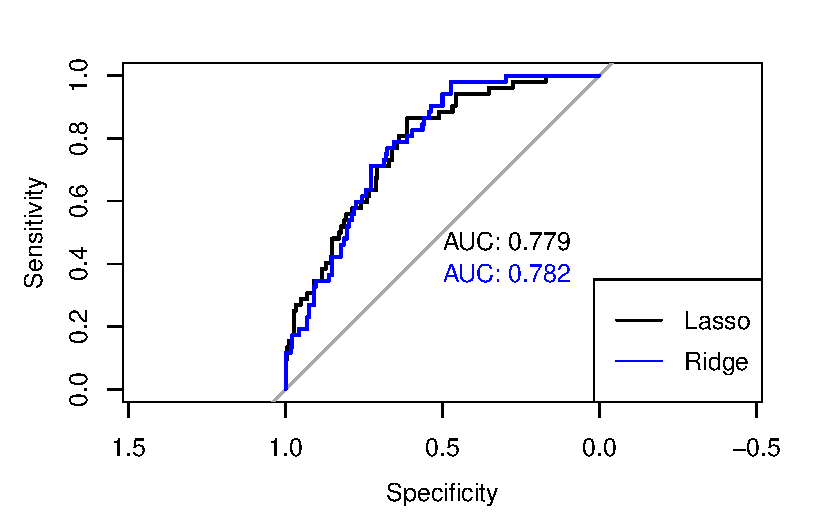
\includegraphics{Untitled_files/figure-pdf/unnamed-chunk-6-1.pdf}

The result shows tha Ridge regression has a higher AUC than Lasso
regression. However, ridge regression do not shrink the coefficients to
zero, and thus can not be used to select variables. There for , we will
also examine the effect of L0 penalty on the model.

\begin{Shaded}
\begin{Highlighting}[]
\FunctionTok{set.seed}\NormalTok{(}\DecValTok{2550}\NormalTok{)}
\NormalTok{subset\_fit }\OtherTok{=} \FunctionTok{L0Learn.cvfit}\NormalTok{(X, Y, }\AttributeTok{nFolds=}\DecValTok{10}\NormalTok{, }\AttributeTok{penalty=}\StringTok{"L0"}\NormalTok{, }\AttributeTok{loss =} \StringTok{\textquotesingle{}Logistic\textquotesingle{}}\NormalTok{)}
\FunctionTok{plot}\NormalTok{(subset\_fit}\SpecialCharTok{$}\NormalTok{cvMeans[[}\DecValTok{1}\NormalTok{]])}
\end{Highlighting}
\end{Shaded}

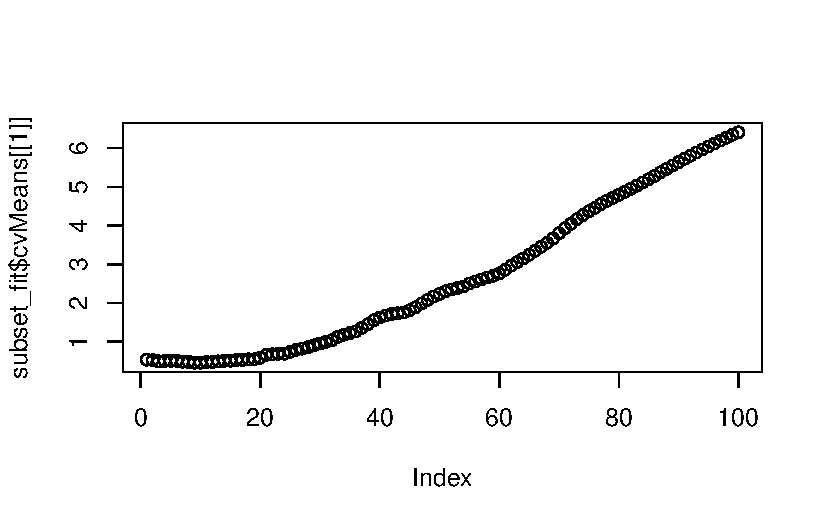
\includegraphics{Untitled_files/figure-pdf/unnamed-chunk-7-1.pdf}

\begin{Shaded}
\begin{Highlighting}[]
\NormalTok{subset\_fit1 }\OtherTok{=} \FunctionTok{L0Learn.cvfit}\NormalTok{(X, Y, }\AttributeTok{nFolds=}\DecValTok{10}\NormalTok{, }\AttributeTok{penalty=}\StringTok{"L0L1"}\NormalTok{, }\AttributeTok{loss =} \StringTok{\textquotesingle{}Logistic\textquotesingle{}}\NormalTok{)}
\FunctionTok{plot}\NormalTok{(}\FunctionTok{sapply}\NormalTok{(subset\_fit1}\SpecialCharTok{$}\NormalTok{cvMeans, mean)) }\CommentTok{\# choose gamma}
\end{Highlighting}
\end{Shaded}

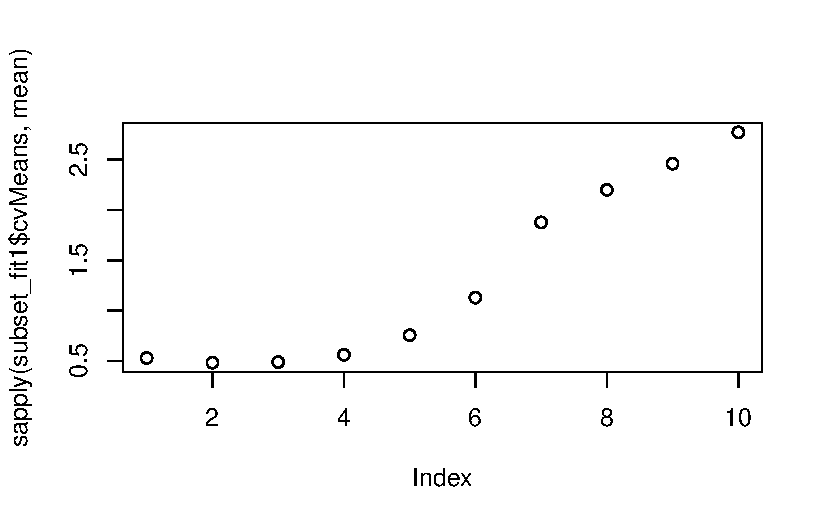
\includegraphics{Untitled_files/figure-pdf/unnamed-chunk-7-2.pdf}

\begin{Shaded}
\begin{Highlighting}[]
\FunctionTok{plot}\NormalTok{(subset\_fit1}\SpecialCharTok{$}\NormalTok{cvMeans[[}\DecValTok{3}\NormalTok{]]) }\CommentTok{\# choose lambda}
\end{Highlighting}
\end{Shaded}

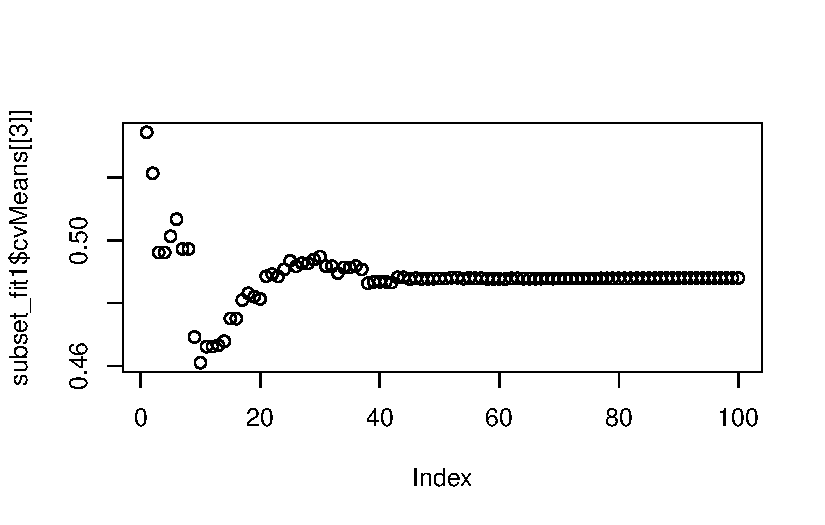
\includegraphics{Untitled_files/figure-pdf/unnamed-chunk-7-3.pdf}

\begin{Shaded}
\begin{Highlighting}[]
\CommentTok{\#coef(subset\_fit, subset\_fit$fit$lambda[[1]][10], 0)}
\CommentTok{\#coef(subset\_fit1, subset\_fit1$fit$lambda[[4]][10], subset\_fit1$fit$gamma[4])}

\NormalTok{auc\_train\_sub0 }\OtherTok{\textless{}{-}} \FunctionTok{roc}\NormalTok{(train\_data}\SpecialCharTok{$}\NormalTok{abst, }\FunctionTok{as.numeric}\NormalTok{(}\FunctionTok{predict}\NormalTok{(subset\_fit, }
                                                          \AttributeTok{type =} \StringTok{"response"}\NormalTok{,}
                                                          \AttributeTok{newx =}\NormalTok{ X, }
\NormalTok{                                                          subset\_fit}\SpecialCharTok{$}\NormalTok{fit}\SpecialCharTok{$}\NormalTok{lambda[[}\DecValTok{1}\NormalTok{]][}\DecValTok{20}\NormalTok{], }
                                                          \DecValTok{0}\NormalTok{)))}
\end{Highlighting}
\end{Shaded}

\begin{verbatim}
Setting levels: control = 0, case = 1
\end{verbatim}

\begin{verbatim}
Setting direction: controls < cases
\end{verbatim}

\begin{Shaded}
\begin{Highlighting}[]
\NormalTok{auc\_train\_sub1 }\OtherTok{\textless{}{-}} \FunctionTok{roc}\NormalTok{(train\_data}\SpecialCharTok{$}\NormalTok{abst, }\FunctionTok{as.numeric}\NormalTok{(}\FunctionTok{predict}\NormalTok{(subset\_fit1, }
                                                          \AttributeTok{type =} \StringTok{"response"}\NormalTok{,}
                                                          \AttributeTok{newx =}\NormalTok{ X, }
\NormalTok{                                                          subset\_fit1}\SpecialCharTok{$}\NormalTok{fit}\SpecialCharTok{$}\NormalTok{lambda[[}\DecValTok{3}\NormalTok{]][}\DecValTok{10}\NormalTok{], }
\NormalTok{                                                          subset\_fit1}\SpecialCharTok{$}\NormalTok{fit}\SpecialCharTok{$}\NormalTok{gamma[}\DecValTok{3}\NormalTok{])))}
\end{Highlighting}
\end{Shaded}

\begin{verbatim}
Setting levels: control = 0, case = 1
Setting direction: controls < cases
\end{verbatim}

\begin{Shaded}
\begin{Highlighting}[]
\FunctionTok{plot.roc}\NormalTok{(auc\_train\_sub0, }\AttributeTok{print.auc=}\ConstantTok{TRUE}\NormalTok{, }\AttributeTok{col =} \StringTok{\textquotesingle{}red\textquotesingle{}}\NormalTok{)}
\FunctionTok{plot.roc}\NormalTok{(auc\_train\_sub1, }\AttributeTok{print.auc=}\ConstantTok{TRUE}\NormalTok{, }\AttributeTok{col =} \StringTok{\textquotesingle{}green\textquotesingle{}}\NormalTok{, }\AttributeTok{add =} \ConstantTok{TRUE}\NormalTok{, }\AttributeTok{print.auc.x =} \FloatTok{0.5}\NormalTok{, }\AttributeTok{print.auc.y =} \FloatTok{0.4}\NormalTok{)}
\FunctionTok{legend}\NormalTok{(}\StringTok{"bottomright"}\NormalTok{, }\AttributeTok{legend =} \FunctionTok{c}\NormalTok{(}\StringTok{"L0"}\NormalTok{, }\StringTok{"L0L1"}\NormalTok{), }\AttributeTok{col =} \FunctionTok{c}\NormalTok{(}\StringTok{"red"}\NormalTok{, }\StringTok{"green"}\NormalTok{), }\AttributeTok{lty =} \DecValTok{1}\NormalTok{)}
\end{Highlighting}
\end{Shaded}

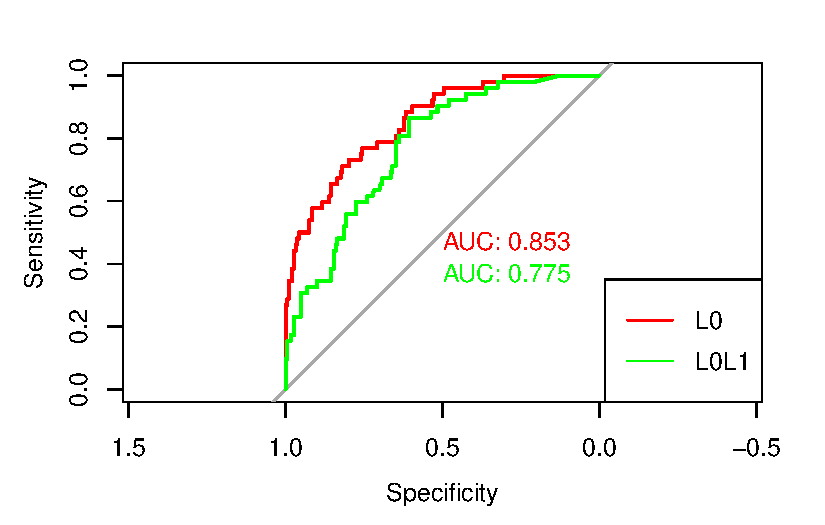
\includegraphics{Untitled_files/figure-pdf/unnamed-chunk-7-4.pdf}

The result shows that L0L1 penalty has the same AUC as L0 penalty within
the train data. We further examine the effect of our models in the test
data.

\begin{Shaded}
\begin{Highlighting}[]
\NormalTok{test\_X }\OtherTok{\textless{}{-}} \FunctionTok{model.matrix}\NormalTok{(abst}\SpecialCharTok{\textasciitilde{}}\NormalTok{ . }\SpecialCharTok{+}\NormalTok{ (NHW }\SpecialCharTok{+}\NormalTok{ ftcd\_score }\SpecialCharTok{+}\NormalTok{ NMR }\SpecialCharTok{+}\NormalTok{ cpd\_ps)}\SpecialCharTok{\^{}}\DecValTok{2} \SpecialCharTok{+}\NormalTok{ Var}\SpecialCharTok{*}\NormalTok{(.) }\SpecialCharTok{+}\NormalTok{ BA}\SpecialCharTok{*}\NormalTok{(.), }
                   \AttributeTok{data =}\NormalTok{ test\_data)}
\NormalTok{test\_X }\OtherTok{\textless{}{-}}\NormalTok{ test\_X[,}\SpecialCharTok{{-}}\DecValTok{1}\NormalTok{]}
\NormalTok{test\_Y }\OtherTok{\textless{}{-}} \FunctionTok{factor}\NormalTok{(test\_data}\SpecialCharTok{$}\NormalTok{abst)}

\NormalTok{auc\_test\_l }\OtherTok{\textless{}{-}} \FunctionTok{roc}\NormalTok{(test\_Y, }\FunctionTok{predict}\NormalTok{(lasso\_fit, }\AttributeTok{type =} \StringTok{"response"}\NormalTok{, }\AttributeTok{newx =}\NormalTok{ test\_X))}
\end{Highlighting}
\end{Shaded}

\begin{verbatim}
Setting levels: control = 0, case = 1
\end{verbatim}

\begin{verbatim}
Warning in roc.default(test_Y, predict(lasso_fit, type = "response", newx =
test_X)): Deprecated use a matrix as predictor. Unexpected results may be
produced, please pass a numeric vector.
\end{verbatim}

\begin{verbatim}
Setting direction: controls < cases
\end{verbatim}

\begin{Shaded}
\begin{Highlighting}[]
\NormalTok{auc\_test\_r }\OtherTok{\textless{}{-}} \FunctionTok{roc}\NormalTok{(test\_Y, }\FunctionTok{predict}\NormalTok{(ridge\_fit, }\AttributeTok{type =} \StringTok{"response"}\NormalTok{, }\AttributeTok{newx =}\NormalTok{ test\_X))}
\end{Highlighting}
\end{Shaded}

\begin{verbatim}
Setting levels: control = 0, case = 1
\end{verbatim}

\begin{verbatim}
Warning in roc.default(test_Y, predict(ridge_fit, type = "response", newx =
test_X)): Deprecated use a matrix as predictor. Unexpected results may be
produced, please pass a numeric vector.
\end{verbatim}

\begin{verbatim}
Setting direction: controls < cases
\end{verbatim}

\begin{Shaded}
\begin{Highlighting}[]
\NormalTok{auc\_test\_sub0 }\OtherTok{\textless{}{-}} \FunctionTok{roc}\NormalTok{(test\_Y, }\FunctionTok{as.numeric}\NormalTok{(}\FunctionTok{predict}\NormalTok{(subset\_fit, }
                                                          \AttributeTok{type =} \StringTok{"response"}\NormalTok{,}
                                                          \AttributeTok{newx =}\NormalTok{ test\_X, }
\NormalTok{                                                          subset\_fit}\SpecialCharTok{$}\NormalTok{fit}\SpecialCharTok{$}\NormalTok{lambda[[}\DecValTok{1}\NormalTok{]][}\DecValTok{20}\NormalTok{], }
                                                          \DecValTok{0}\NormalTok{)))}
\end{Highlighting}
\end{Shaded}

\begin{verbatim}
Setting levels: control = 0, case = 1
\end{verbatim}

\begin{verbatim}
Setting direction: controls < cases
\end{verbatim}

\begin{Shaded}
\begin{Highlighting}[]
\NormalTok{auc\_test\_sub1 }\OtherTok{\textless{}{-}} \FunctionTok{roc}\NormalTok{(test\_Y, }\FunctionTok{as.numeric}\NormalTok{(}\FunctionTok{predict}\NormalTok{(subset\_fit1, }
                                                          \AttributeTok{type =} \StringTok{"response"}\NormalTok{,}
                                                          \AttributeTok{newx =}\NormalTok{ test\_X, }
\NormalTok{                                                          subset\_fit1}\SpecialCharTok{$}\NormalTok{fit}\SpecialCharTok{$}\NormalTok{lambda[[}\DecValTok{3}\NormalTok{]][}\DecValTok{10}\NormalTok{], }
\NormalTok{                                                          subset\_fit1}\SpecialCharTok{$}\NormalTok{fit}\SpecialCharTok{$}\NormalTok{gamma[}\DecValTok{3}\NormalTok{])))}
\end{Highlighting}
\end{Shaded}

\begin{verbatim}
Setting levels: control = 0, case = 1
Setting direction: controls < cases
\end{verbatim}

\begin{Shaded}
\begin{Highlighting}[]
\FunctionTok{plot.roc}\NormalTok{(auc\_test\_l, }\AttributeTok{print.auc=}\ConstantTok{TRUE}\NormalTok{, }\AttributeTok{col =} \StringTok{\textquotesingle{}black\textquotesingle{}}\NormalTok{)}
\FunctionTok{plot.roc}\NormalTok{(auc\_test\_r, }\AttributeTok{print.auc=}\ConstantTok{TRUE}\NormalTok{, }\AttributeTok{col =} \StringTok{\textquotesingle{}blue\textquotesingle{}}\NormalTok{, }\AttributeTok{add =} \ConstantTok{TRUE}\NormalTok{, }\AttributeTok{print.auc.x =} \FloatTok{0.5}\NormalTok{, }\AttributeTok{print.auc.y =} \FloatTok{0.4}\NormalTok{)}
\FunctionTok{plot.roc}\NormalTok{(auc\_test\_sub0, }\AttributeTok{print.auc=}\ConstantTok{TRUE}\NormalTok{, }\AttributeTok{col =} \StringTok{\textquotesingle{}red\textquotesingle{}}\NormalTok{, }\AttributeTok{add =} \ConstantTok{TRUE}\NormalTok{, }\AttributeTok{print.auc.x =} \FloatTok{0.5}\NormalTok{, }\AttributeTok{print.auc.y =} \FloatTok{0.3}\NormalTok{)}
\FunctionTok{plot.roc}\NormalTok{(auc\_test\_sub1, }\AttributeTok{print.auc=}\ConstantTok{TRUE}\NormalTok{, }\AttributeTok{col =} \StringTok{\textquotesingle{}green\textquotesingle{}}\NormalTok{, }\AttributeTok{add =} \ConstantTok{TRUE}\NormalTok{, }\AttributeTok{print.auc.x =} \FloatTok{0.5}\NormalTok{, }\AttributeTok{print.auc.y =} \FloatTok{0.2}\NormalTok{)}
\FunctionTok{legend}\NormalTok{(}\StringTok{"bottomright"}\NormalTok{, }\AttributeTok{legend =} \FunctionTok{c}\NormalTok{(}\StringTok{"Lasso"}\NormalTok{, }\StringTok{"Ridge"}\NormalTok{, }\StringTok{"L0"}\NormalTok{, }\StringTok{"L0L1"}\NormalTok{), }\AttributeTok{col =} \FunctionTok{c}\NormalTok{(}\StringTok{"black"}\NormalTok{, }\StringTok{"blue"}\NormalTok{,}\StringTok{"red"}\NormalTok{, }\StringTok{"green"}\NormalTok{), }\AttributeTok{lty =} \DecValTok{1}\NormalTok{)}
\end{Highlighting}
\end{Shaded}

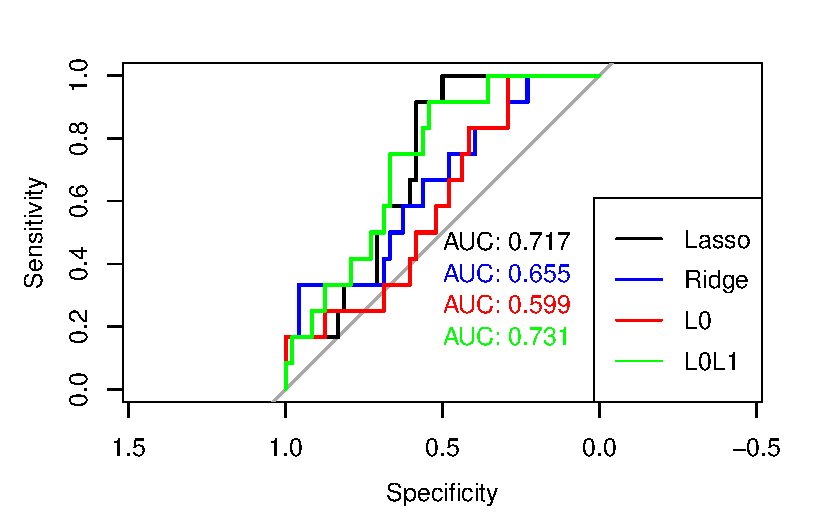
\includegraphics{Untitled_files/figure-pdf/unnamed-chunk-8-1.pdf}

subset selection with ridge regression has the highest AUC in the test
data. It is worth to notice that lasso regression, eventhough have a
lower AUC than subset selection with ridge regression, performs better
for the purpose of hight sensitivity.

\begin{Shaded}
\begin{Highlighting}[]
\NormalTok{coef\_l0 }\OtherTok{\textless{}{-}} \FunctionTok{coef}\NormalTok{(subset\_fit1, subset\_fit1}\SpecialCharTok{$}\NormalTok{fit}\SpecialCharTok{$}\NormalTok{lambda[[}\DecValTok{3}\NormalTok{]][}\DecValTok{10}\NormalTok{], subset\_fit1}\SpecialCharTok{$}\NormalTok{fit}\SpecialCharTok{$}\NormalTok{gamma[}\DecValTok{3}\NormalTok{])}
\NormalTok{coef\_l0\_names }\OtherTok{\textless{}{-}} \FunctionTok{row.names}\NormalTok{(}\FunctionTok{coef}\NormalTok{(lasso\_fit))}
\NormalTok{coef\_l0\_index }\OtherTok{\textless{}{-}} \FunctionTok{which}\NormalTok{(coef\_l0 }\SpecialCharTok{!=} \DecValTok{0}\NormalTok{)}
\NormalTok{coef\_l0 }\OtherTok{\textless{}{-}}\NormalTok{ coef\_l0[coef\_l0\_index]}
\NormalTok{coef\_l0\_names }\OtherTok{\textless{}{-}}\NormalTok{ coef\_l0\_names[coef\_l0\_index]}

\CommentTok{\#coef\_lasso \textless{}{-} coef(lasso\_fit, s = "lambda.min")}
\CommentTok{\#coef\_lasso\_names \textless{}{-} row.names(coef\_lasso)}
\CommentTok{\#coef\_lasso\_index \textless{}{-} which(coef\_lasso != 0)}
\CommentTok{\#coef\_lasso \textless{}{-} coef\_lasso[coef\_lasso\_index]}
\CommentTok{\#coef\_lasso\_names \textless{}{-} coef\_lasso\_names[coef\_lasso\_index]}

\NormalTok{coef\_tbl }\OtherTok{\textless{}{-}} \FunctionTok{data.frame}\NormalTok{(coef\_l0\_names, coef\_l0)}
\end{Highlighting}
\end{Shaded}

The table shows the coefficients of the subset selection with L0L1
penalty. The result shows that the interaction term of NHW and
ftcd\_score has the highest coefficient, which means that the
interaction term has the most significant effect on the outcome.



\end{document}
